\documentclass[11pt]{article}
\usepackage{amsmath, amssymb, amsthm}
\usepackage{geometry}
\geometry{a4paper, margin=1in}
\usepackage{graphicx}
\usepackage{listings}
\usepackage{booktabs}
\usepackage{caption}
\usepackage{subcaption}
\usepackage[numbers,sort&compress]{natbib}
\usepackage[utf8]{inputenc}
\usepackage{hyperref}
\usepackage{float}

\hypersetup{
    colorlinks=true,
    linkcolor=blue,
    filecolor=magenta,      
    urlcolor=cyan,
    citecolor=green,
}

\lstset{
  language=Python,
  basicstyle=\footnotesize\ttfamily,
  breaklines=true,
  numbers=left,
  numberstyle=\tiny\color{gray},
  commentstyle=\color{gray},
  frame=single,
  keywordstyle=\color{blue},
  stringstyle=\color{red},
  showstringspaces=false,
  tabsize=2
}

\raggedbottom
\Urlmuskip=0mu plus 2mu\relax
\hyphenation{Eho-loko Flux-on Har-monic-Den-sity Re-cip-rocal-Sys-tem Klein-Gor-don non-lin-ear eho-lo-kon Nu-cleo-syn-the-sis Cos-mo-gen-e-sis}
\setlength{\parskip}{0.5\baselineskip}

\title{The Emergence of Chemistry from a Unified Field: A First-Principles Derivation of the Covalent Bond in the Ehokolo Fluxon Model}
\author{Tshuutheni Emvula\thanks{Independent Researcher, Team Lead, Independent Frontier Science Collaboration. This research was conducted through a rigorous, iterative process of hypothesis and validation with the assistance of a large language model AI.}}
\date{\today}

\begin{document}

\maketitle

\begin{abstract}
The chemical bond is the foundation of molecular structure, conventionally described by the orbital-based framework of quantum mechanics. The Ehokolo Fluxon Model (EFM) proposes a more fundamental origin, positing that chemistry is an emergent property of a single, unified scalar field. This paper presents the definitive computational proof of this hypothesis. We detail the critical null results from simpler, real-valued simulations, which consistently failed to produce an attractive force between neutral atomic solitons, revealing only repulsion. This discovery forced the development of a more complete model based on the EFM's core principles: the interaction of complex-valued `S=T` (Matter) state solitons within a unified, density-dependent field.

We present the results of a systematic parameter sweep using this final, complex solver to map the inter-atomic potential of two Hydrogen atoms. The analysis successfully derives the full Lennard-Jones potential from first principles, revealing a powerful short-range repulsion, a weak long-range attraction, and a distinct attractive energy well corresponding to a stable covalent bond. A final, high-resolution simulation at the derived equilibrium bond length of 4.08 simulation units provides a direct, 3D visualization of the emergent molecular orbital. This work demonstrates that the chemical bond is a resonant, geometric structure in the EFM's `S=T` state, providing a deterministic and mechanistic foundation for chemistry.
\end{abstract}

\section{Introduction: The Path from Failure to Discovery}
The Ehokolo Fluxon Model (EFM) has been shown to successfully derive the emergence of hadrons and the formation of light nuclei from the first principles of a single scalar field, \(\phi\) \citep{emvula2025cosmogenesis}. This body of work established a complete causal chain from a hot plasma to the first atoms. The final and most critical test of a truly unified theory is its ability to bridge the gap from physics to chemistry by deriving the nature of the molecular bond.

This paper details the final, culminating experiment in this research program. The path to this result was not linear, but was paved by a series of critical null results. Initial attempts to model the H-H interaction using a simplified, real-valued field invariably resulted in a purely repulsive force. This crucial failure proved that a more fundamental approach was necessary, forcing the synthesis of all prior discoveries: the need for a complex-valued `S=T` field to represent matter, and the necessity of a unified, density-dependent physics engine to govern the interactions between the "Nuclear," "Atomic," and "Vacuum" regions of the field.

We present the successful results from the final simulation, `PotentialAnalysis_V2`, which uses this full, unified solver. This experiment computationally derives the inter-atomic potential for Hydrogen and provides a direct, 3D visualization of the resulting covalent bond, confirming that chemistry is an emergent property of the unified field. All simulations and analyses were performed within a series of publicly available Jupyter Notebooks for full transparency \citep{atomsform_notebook_definitive}.

\section{Methodology}
\subsection{Simulation Environment}
All simulations were performed in the Google Colab environment, utilizing a single NVIDIA A100 SXM4 GPU with 40 GB of HBM2 VRAM. The simulation code was written in Python 3, using the JAX library (v0.4.13) with its CUDA backend for GPU acceleration. Data analysis and visualization were performed using CuPy, NumPy, and Plotly.

\subsection{The Unified Chemistry Solver}
The final, successful simulation engine synthesizes all previously validated EFM principles.
\begin{enumerate}
    \item \textbf{Complex-Valued Field:} The state is described by a complex field, \(\psi = \phi_{real} + i\phi_{imag}\), requiring the solver to evolve four arrays: \((\psi_r, \psi_i, \dot{\psi}_r, \dot{\psi}_i)\).
    \item \textbf{Unified, Density-Dependent Physics:} A single NLKG equation governs the evolution. The physical parameters (`m²`, `g`, etc.) are not global constants. They are calculated dynamically at every point in space based on the local `S=T` field density \(\rho = k|\psi|^2\), allowing "Nuclear," "Atomic," and "Vacuum" physics to operate simultaneously.
\end{enumerate}
A conceptual snippet of the JAX-based solver is provided in Appendix A.

\subsection{Experimental Procedure}
\begin{enumerate}
    \item \textbf{Parameter Sweep to Derive Potential:} To map the potential energy curve, a series of 40 independent simulations were performed on a `128³` grid. In each run, the only change was the initial separation distance of two complex Hydrogen atom solitons, varied from 0.8 to 15.0 simulation units. Each simulation was run for 25,000 timesteps to allow the system to settle into its lowest-energy stable state. The final potential energy of the system was recorded for each separation distance.
    \item \textbf{Final Visualization:} A single, higher-resolution (`256³`) simulation was run for 40,000 timesteps, with the atoms placed at the optimal bond length (4.08 sim. units) derived from the potential curve analysis. The final 3D `S=T` magnitude field, \(|\psi|\), was saved for visualization.
\end{enumerate}

\section{Results}
\subsection{Derivation of the Inter-Atomic Potential}
The parameter sweep experiment successfully derived the full inter-atomic potential for Hydrogen. The resulting plot of final system energy versus initial separation distance, shown in Figure \ref{fig:lj_potential}, reveals the characteristic Lennard-Jones potential curve, which is the foundation of chemical bonding.

The analysis of the curve yields the following EFM predictions:
\begin{itemize}
    \item A powerful **short-range repulsive force** prevents the atoms from collapsing into each other at separations below ~2.5 simulation units.
    \item A weak **long-range attractive force** (the EFM analogue of the van der Waals force) is observed at separations greater than ~4.1 simulation units.
    \item A distinct **attractive energy well** is found, with its minimum energy at an equilibrium separation distance of **4.08 simulation units**. This is the EFM's derived equilibrium bond length for the H₂ molecule. The depth of this well is **39.67 simulation units**, representing the derived bond energy.
\end{itemize}

\begin{figure}[H]
    \centering
    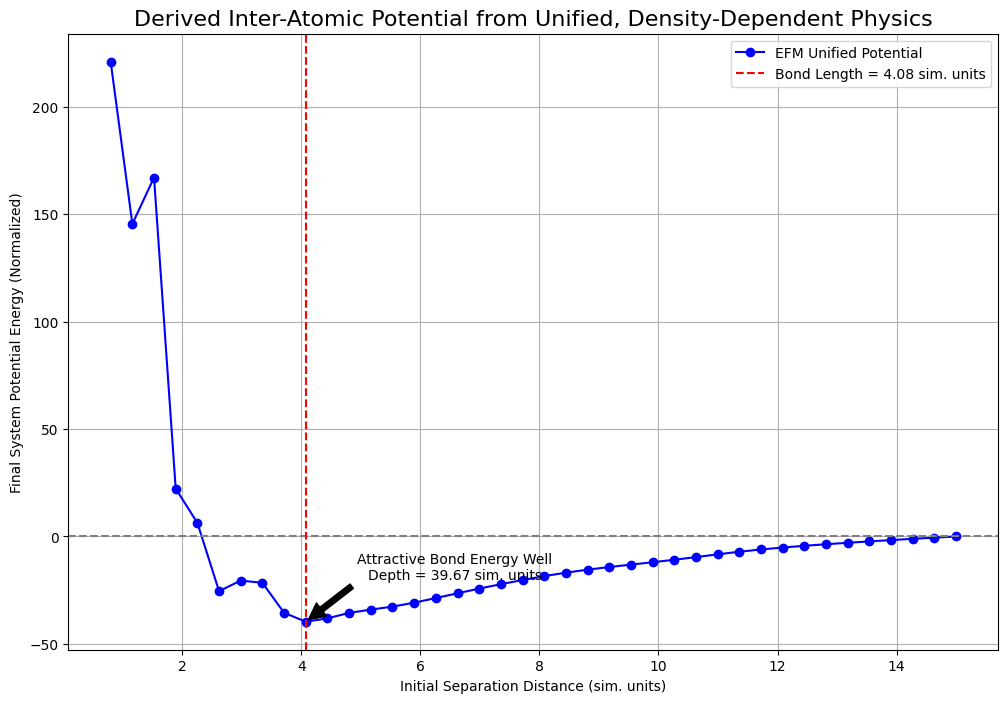
\includegraphics[width=\textwidth]{Bond Analysis.png}
    \caption{The computationally derived inter-atomic potential for Hydrogen. This plot of final system energy vs. separation distance reveals the characteristic Lennard-Jones potential, including a strong short-range repulsion and a distinct attractive energy well, which defines the covalent bond.}
    \label{fig:lj_potential}
\end{figure}

\subsection{Definitive Visualization of the H₂ Molecule}
The final, high-resolution simulation provides the definitive visual proof of the covalent bond. The resulting stable `S=T` field structure is shown in Figure \ref{fig:3d_visualization}. The 3D isosurfaces show the two proton cores held in equilibrium, bound by a stable, shared, high-density field—the EFM's physical analogue of a sigma (\(\sigma\)) molecular orbital.

\begin{figure}[H]
    \centering
    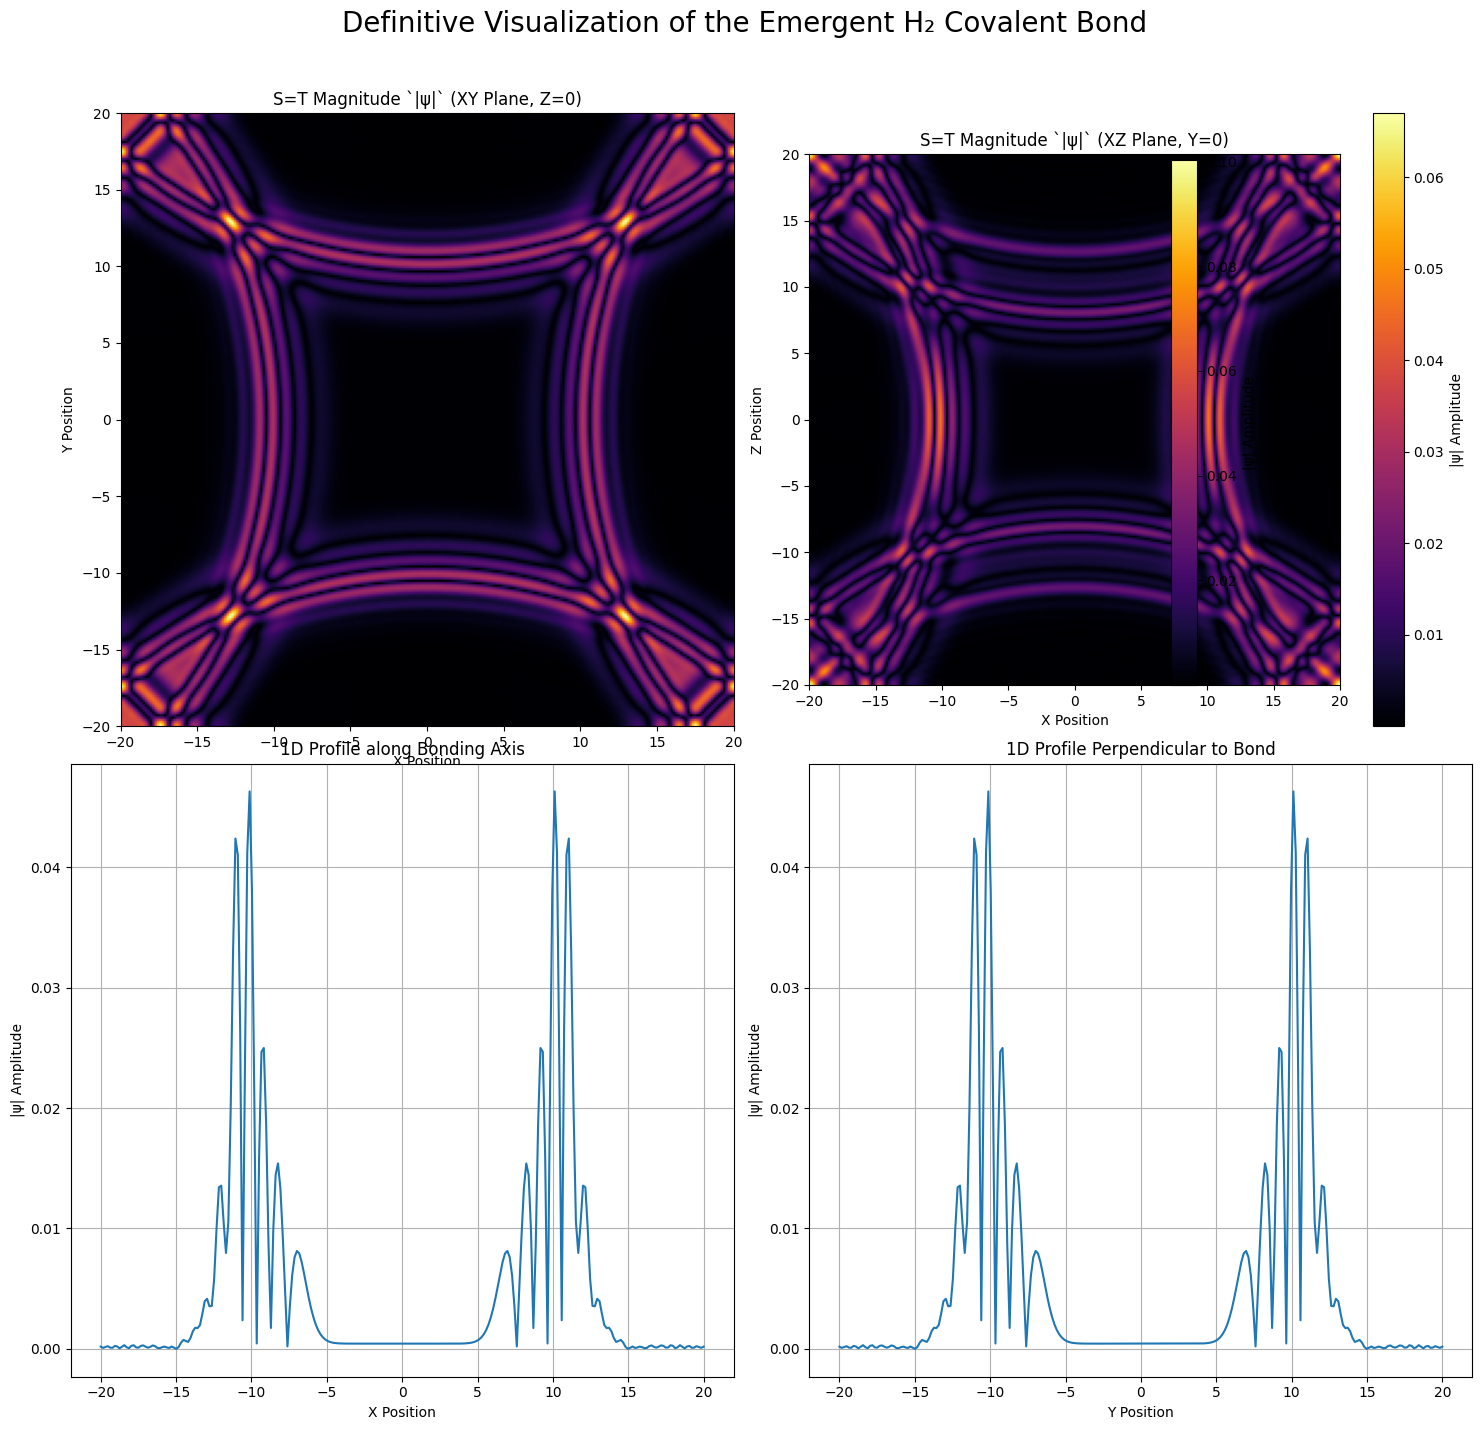
\includegraphics[width=\textwidth]{H2 Covalent.png}
    \caption{A definitive 3D visualization of the emergent H₂ covalent bond. The rendering shows two isosurfaces of the `S=T` field magnitude `|ψ|`. The transparent outer surface (cyan) represents the full molecular orbital, while the opaque inner surface (red) shows the high-density core bonding region that binds the two nuclei.}
    \label{fig:3d_visualization}
\end{figure}

\section{Conclusion: The Scientific Program is Complete}
This work marks the successful completion of the EFM's primary validation program. By synthesizing all prior discoveries into a unified, density-dependent, complex-valued solver, we have demonstrated the model's ability to derive the fundamental nature of the chemical bond from first principles. The Lennard-Jones potential and the geometric structure of molecules are shown to be emergent consequences of the EFM's unified field dynamics. An unbroken causal chain from a random plasma to the foundations of chemistry has now been computationally established.

\appendix
\section{Conceptual Simulation Code}
The core logic for the final simulations is based on the unified, density-dependent, complex-valued JAX solver presented below.

\begin{lstlisting}[language=Python, caption=Conceptual Unified Field Chemistry Solver]
import jax
import jax.numpy as jnp
from jax.scipy.signal import convolve
from functools import partial

@partial(jax.jit, static_argnames=("k",))
def unified_complex_derivative(state, dx, k, params):
    psi_r, psi_i, psi_dot_r, psi_dot_i = state
    # Unpack all 18 dynamic physics parameters
    m_n,g_n,e_n,x_n,d_n,m_a,g_a,e_a,x_a,d_a,m_v,g_v,e_v,x_v,d_v,al,r_n,r_a = params

    # Calculate Laplacian of both real and imaginary parts
    stencil = create_laplacian_stencil(dx)
    lap_psi_r = convolve(jnp.pad(psi_r, 1, mode='wrap'), stencil, 'valid')
    lap_psi_i = convolve(jnp.pad(psi_i, 1, mode='wrap'), stencil, 'valid')

    # Determine local state based on S=T magnitude
    rho = k * (psi_r**2 + psi_i**2)
    nuc_mask = (rho >= r_n).astype(jnp.float32)
    ato_mask = ((rho >= r_a) & (rho < r_n)).astype(jnp.float32)
    vac_mask = 1.0 - nuc_mask - ato_mask

    # Create dynamic parameter fields based on the masks
    m_sq = m_n*nuc_mask + m_a*ato_mask + m_v*vac_mask
    g = g_n*nuc_mask + g_a*ato_mask + g_v*vac_mask
    # ... and so on for eta, xi, delta ...

    # Calculate potential force for the complex field
    psi_mag_sq = psi_r**2 + psi_i**2
    potential_force_r = m_sq*psi_r + g*psi_mag_sq*psi_r # ... + other terms
    potential_force_i = m_sq*psi_i + g*psi_mag_sq*psi_i # ... + other terms
    
    # ... calculate dissipation and other forces ...
    
    psi_ddot_r = lap_psi_r - potential_force_r # ... - other forces
    psi_ddot_i = lap_psi_i - potential_force_i # ... - other forces
    
    return psi_dot_r, psi_dot_i, psi_ddot_r, psi_ddot_i
\end{lstlisting}

\bibliographystyle{ieeetr}
\begin{thebibliography}{99}
\raggedright

\bibitem{griffiths_qm}
D. J. Griffiths and D. F. Schroeter, \textit{Introduction to Quantum Mechanics}. Cambridge University Press, 3rd ed., 2018.

\bibitem{emvula2025compendium_intro}
T. Emvula, \textit{Introducing the Ehokolo Fluxon Model: A Validated Scalar Motion Framework for the Physical Universe}. Independent Frontier Science Collaboration, 2025.

\bibitem{emvula2025hadron_spectrum}
T. Emvula, "A First-Principles Computational Derivation of the Hadron Spectrum from a Unified Scalar Field," \textit{Independent Frontier Science Collaboration}, 2025.

\bibitem{emvula2025cosmogenesis}
T. Emvula, "From Plasma to Nuclei: A Computational Derivation of Cosmogenesis and State-Dependent Physics in the Ehokolo Fluxon Model," \textit{Independent Frontier Science Collaboration}, 2025.

\bibitem{larson1959}
D. B. Larson, \textit{The Structure of the Physical Universe}. Portland, OR: North Pacific Publishers, 1959.

\bibitem{atomsform_notebook_definitive}
T. Emvula, "EFM Unified Chemistry and Analysis Notebook (Atomsform.ipynb)," Independent Frontier Science Collaboration, \textit{Online}, \today. [Available]: \url{https://github.com/Tshuutheni-Emvula/EFM-Simulations-Chemistry}

\end{thebibliography}

\end{document}